\documentclass[12pt,a4paper]{article}

\usepackage[utf8]{inputenc}
\usepackage[english]{babel}
\usepackage{graphicx}
\usepackage{float}
\usepackage{amsmath}
\usepackage{hyperref}
\usepackage{listings}
\usepackage{xcolor}
\usepackage{booktabs}
\usepackage{subcaption}
\usepackage[margin=1in]{geometry}
\usepackage{cite}

\lstset{
    basicstyle=\ttfamily\small,
    keywordstyle=\color{blue},
    commentstyle=\color{green!60!black},
    stringstyle=\color{red},
    numbers=left,
    numberstyle=\tiny\color{gray},
    stepnumber=1,
    numbersep=5pt,
    backgroundcolor=\color{white},
    showspaces=false,
    showstringspaces=false,
    showtabs=false,
    frame=single,
    tabsize=2,
    captionpos=b,
    breaklines=true,
    breakatwhitespace=false,
    escapeinside={\%*}{*)},
    language=C++
}

\title{Real-time video processing\\
\large Visual Computing Assignment}
\author{Mads Pagh\\
Student ID: 202208375\\
Aarhus University}
\date{\today}

\begin{document}

\maketitle
\newpage

\tableofcontents
\newpage

\section{Introduction}
In this report an analysis of real-time image processing performance using OpenCV and OpenGL is presented. The project implements various image filters and geometric transformations, comparing CPU and GPU execution across different resolutions.

\subsection{Objectives}
\begin{itemize}
    \item Implement real-time image filters using OpenCV (CPU) and OpenGL shaders (GPU)
    \item Compare performance between CPU and GPU execution
    \item Analyze the impact of resolution on processing performance
    \item Evaluate the overhead of geometric transformations
\end{itemize}

\section{Methodology}

\subsection{System Architecture}
The system consists of three main components:
\begin{itemize}
    \item \textbf{Video Capture}: OpenCV VideoCapture for webcam input
    \item \textbf{Processing Pipeline}: CPU (OpenCV) and GPU (OpenGL/GLFW) implementations
    \item \textbf{Rendering}: OpenGL for display and GPU acceleration
\end{itemize}


\subsection{Implemented Filters}
Six different image filters were implemented:
\begin{enumerate}
    \item \textbf{None} - The frames are passed through without any filtering
    \item \textbf{Grayscale} - Color to grayscale conversion
    \item \textbf{Gaussian Blur} - 5x5 kernel blur
    \item \textbf{Edge Detection} - Sobel operator
    \item \textbf{Pixelation} - 10x10 pixel blocks
    \item \textbf{Comic Art} - Edge detection combined with color quantization
\end{enumerate}

\subsection{Geometric Transformations}
Five transformation configurations were tested:
\begin{enumerate}
    \item No Transform (baseline)
    \item Translation only ($t_x = 0.3, t_y = 0.2$)
    \item Scale only ($s = 1.5$)
    \item Rotation only ($\theta = 25 \text{ degrees}$)
    \item Combined ($t_x = 0.2, t_y = -0.15, s = 1.3, \theta = 15 \text{ degrees}$)
\end{enumerate}

\subsection{Test Resolutions}
Three resolutions were benchmarked:
\begin{itemize}
    \item VGA: 640×480 (307,200 pixels)
    \item HD: 1280×720 (921,600 pixels)
    \item Full HD: 1920×1080 (2,073,600 pixels)
\end{itemize}

\subsection{Benchmarking Procedure}
\begin{itemize}
    \item Each test configuration ran for 50 frames (transforms) or 50 frames (resolution) due to hardware limitations
    \item Frame times were measured using high-resolution clock
    \item Average FPS and frame time statistics were calculated
    \item Tests were automated to ensure consistency, could have been done manually, but fear of human error and tendency to forget configurations made automation preferable
\end{itemize}

\section{Results}

\subsection{Transform Benchmark Results}

\subsubsection{GPU vs CPU Performance}
\begin{figure}[H]
    \centering
    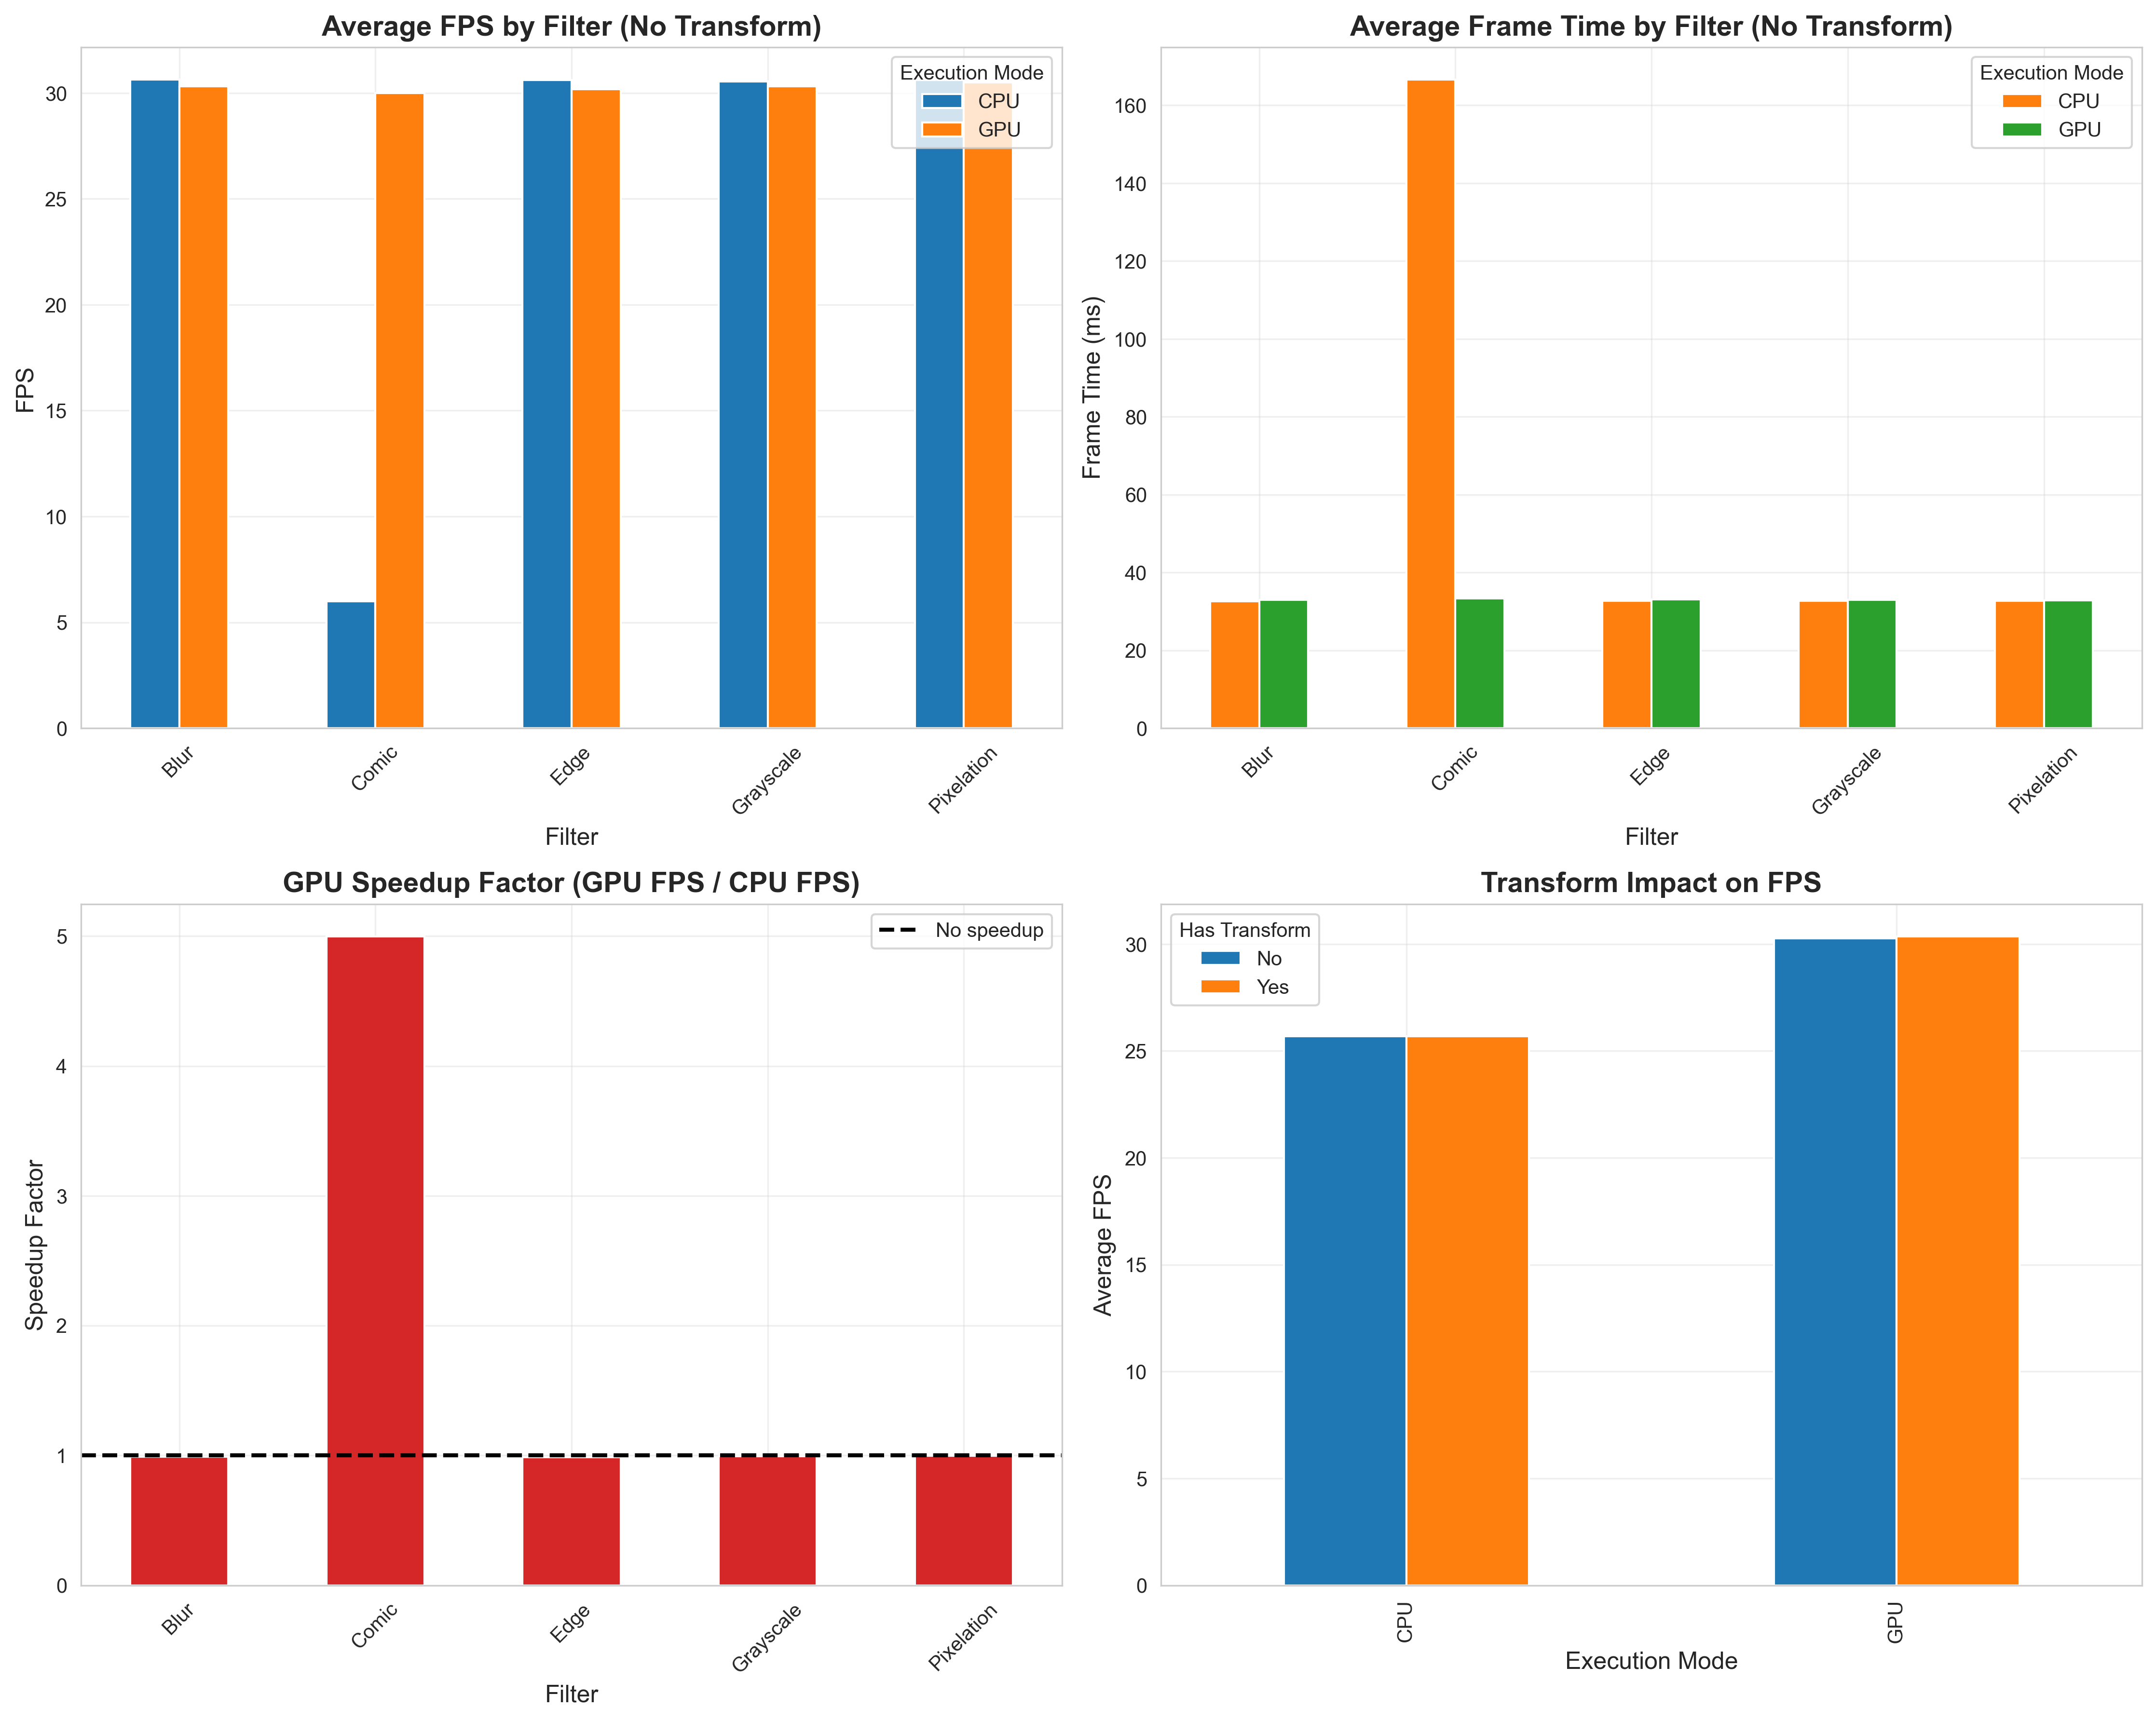
\includegraphics[width=0.9\textwidth]{../data/plots/performance_comparison_transforms.png}
    \caption{Performance comparison across filters and execution modes}
    \label{fig:transform_comparison}
\end{figure}

% TODO: Add analysis text here

\subsubsection{Transform Impact}
\begin{figure}[H]
    \centering
    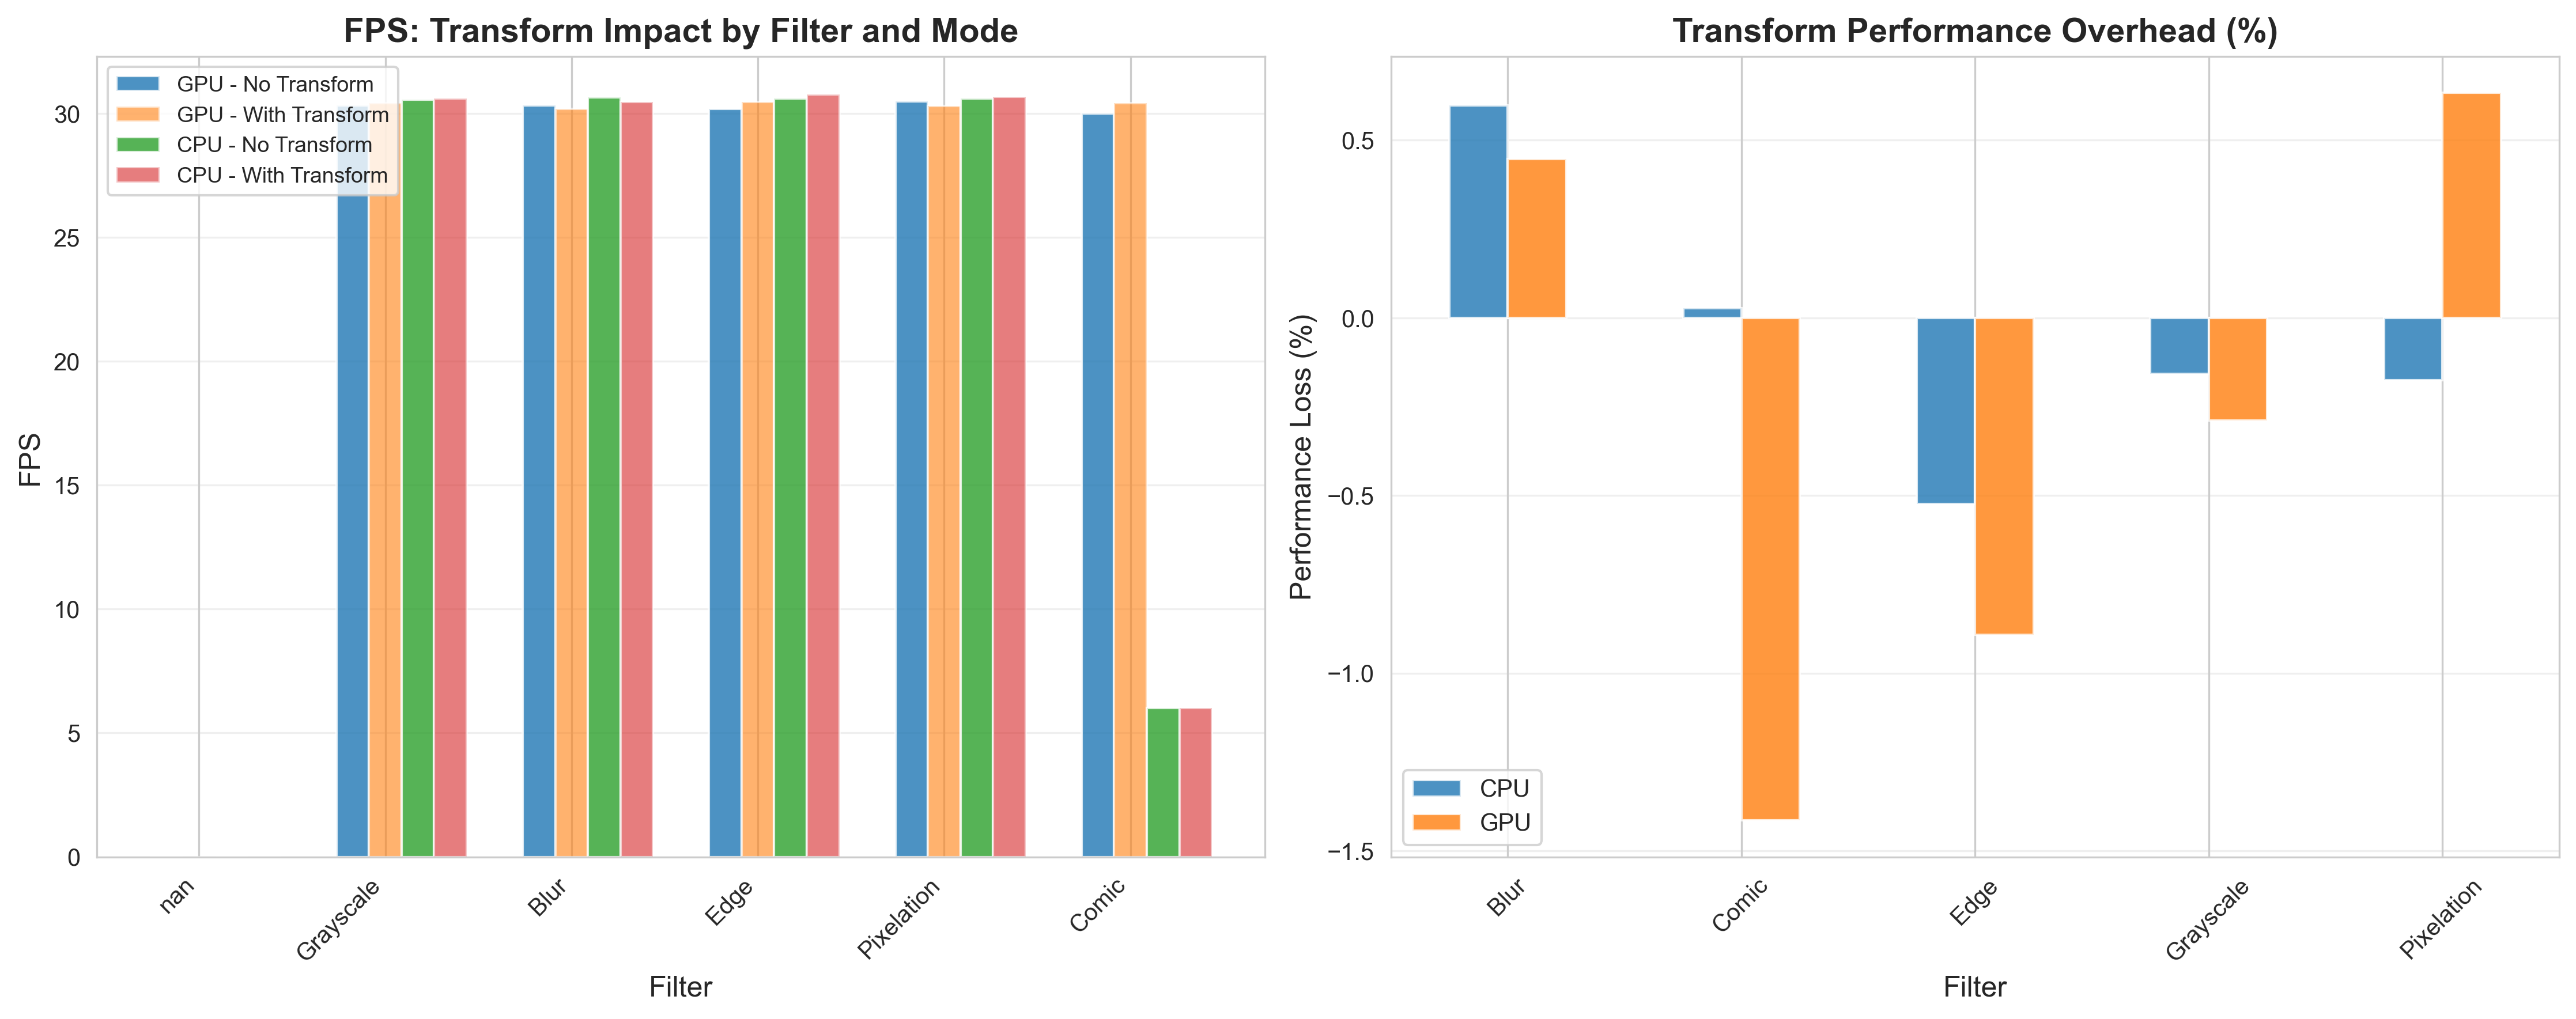
\includegraphics[width=0.9\textwidth]{../data/plots/transform_comparison.png}
    \caption{Impact of geometric transformations on performance}
    \label{fig:transform_impact}
\end{figure}

% TODO: Add analysis text here

\subsection{Resolution Benchmark Results}

\subsubsection{Resolution Scaling}
\begin{figure}[H]
    \centering
    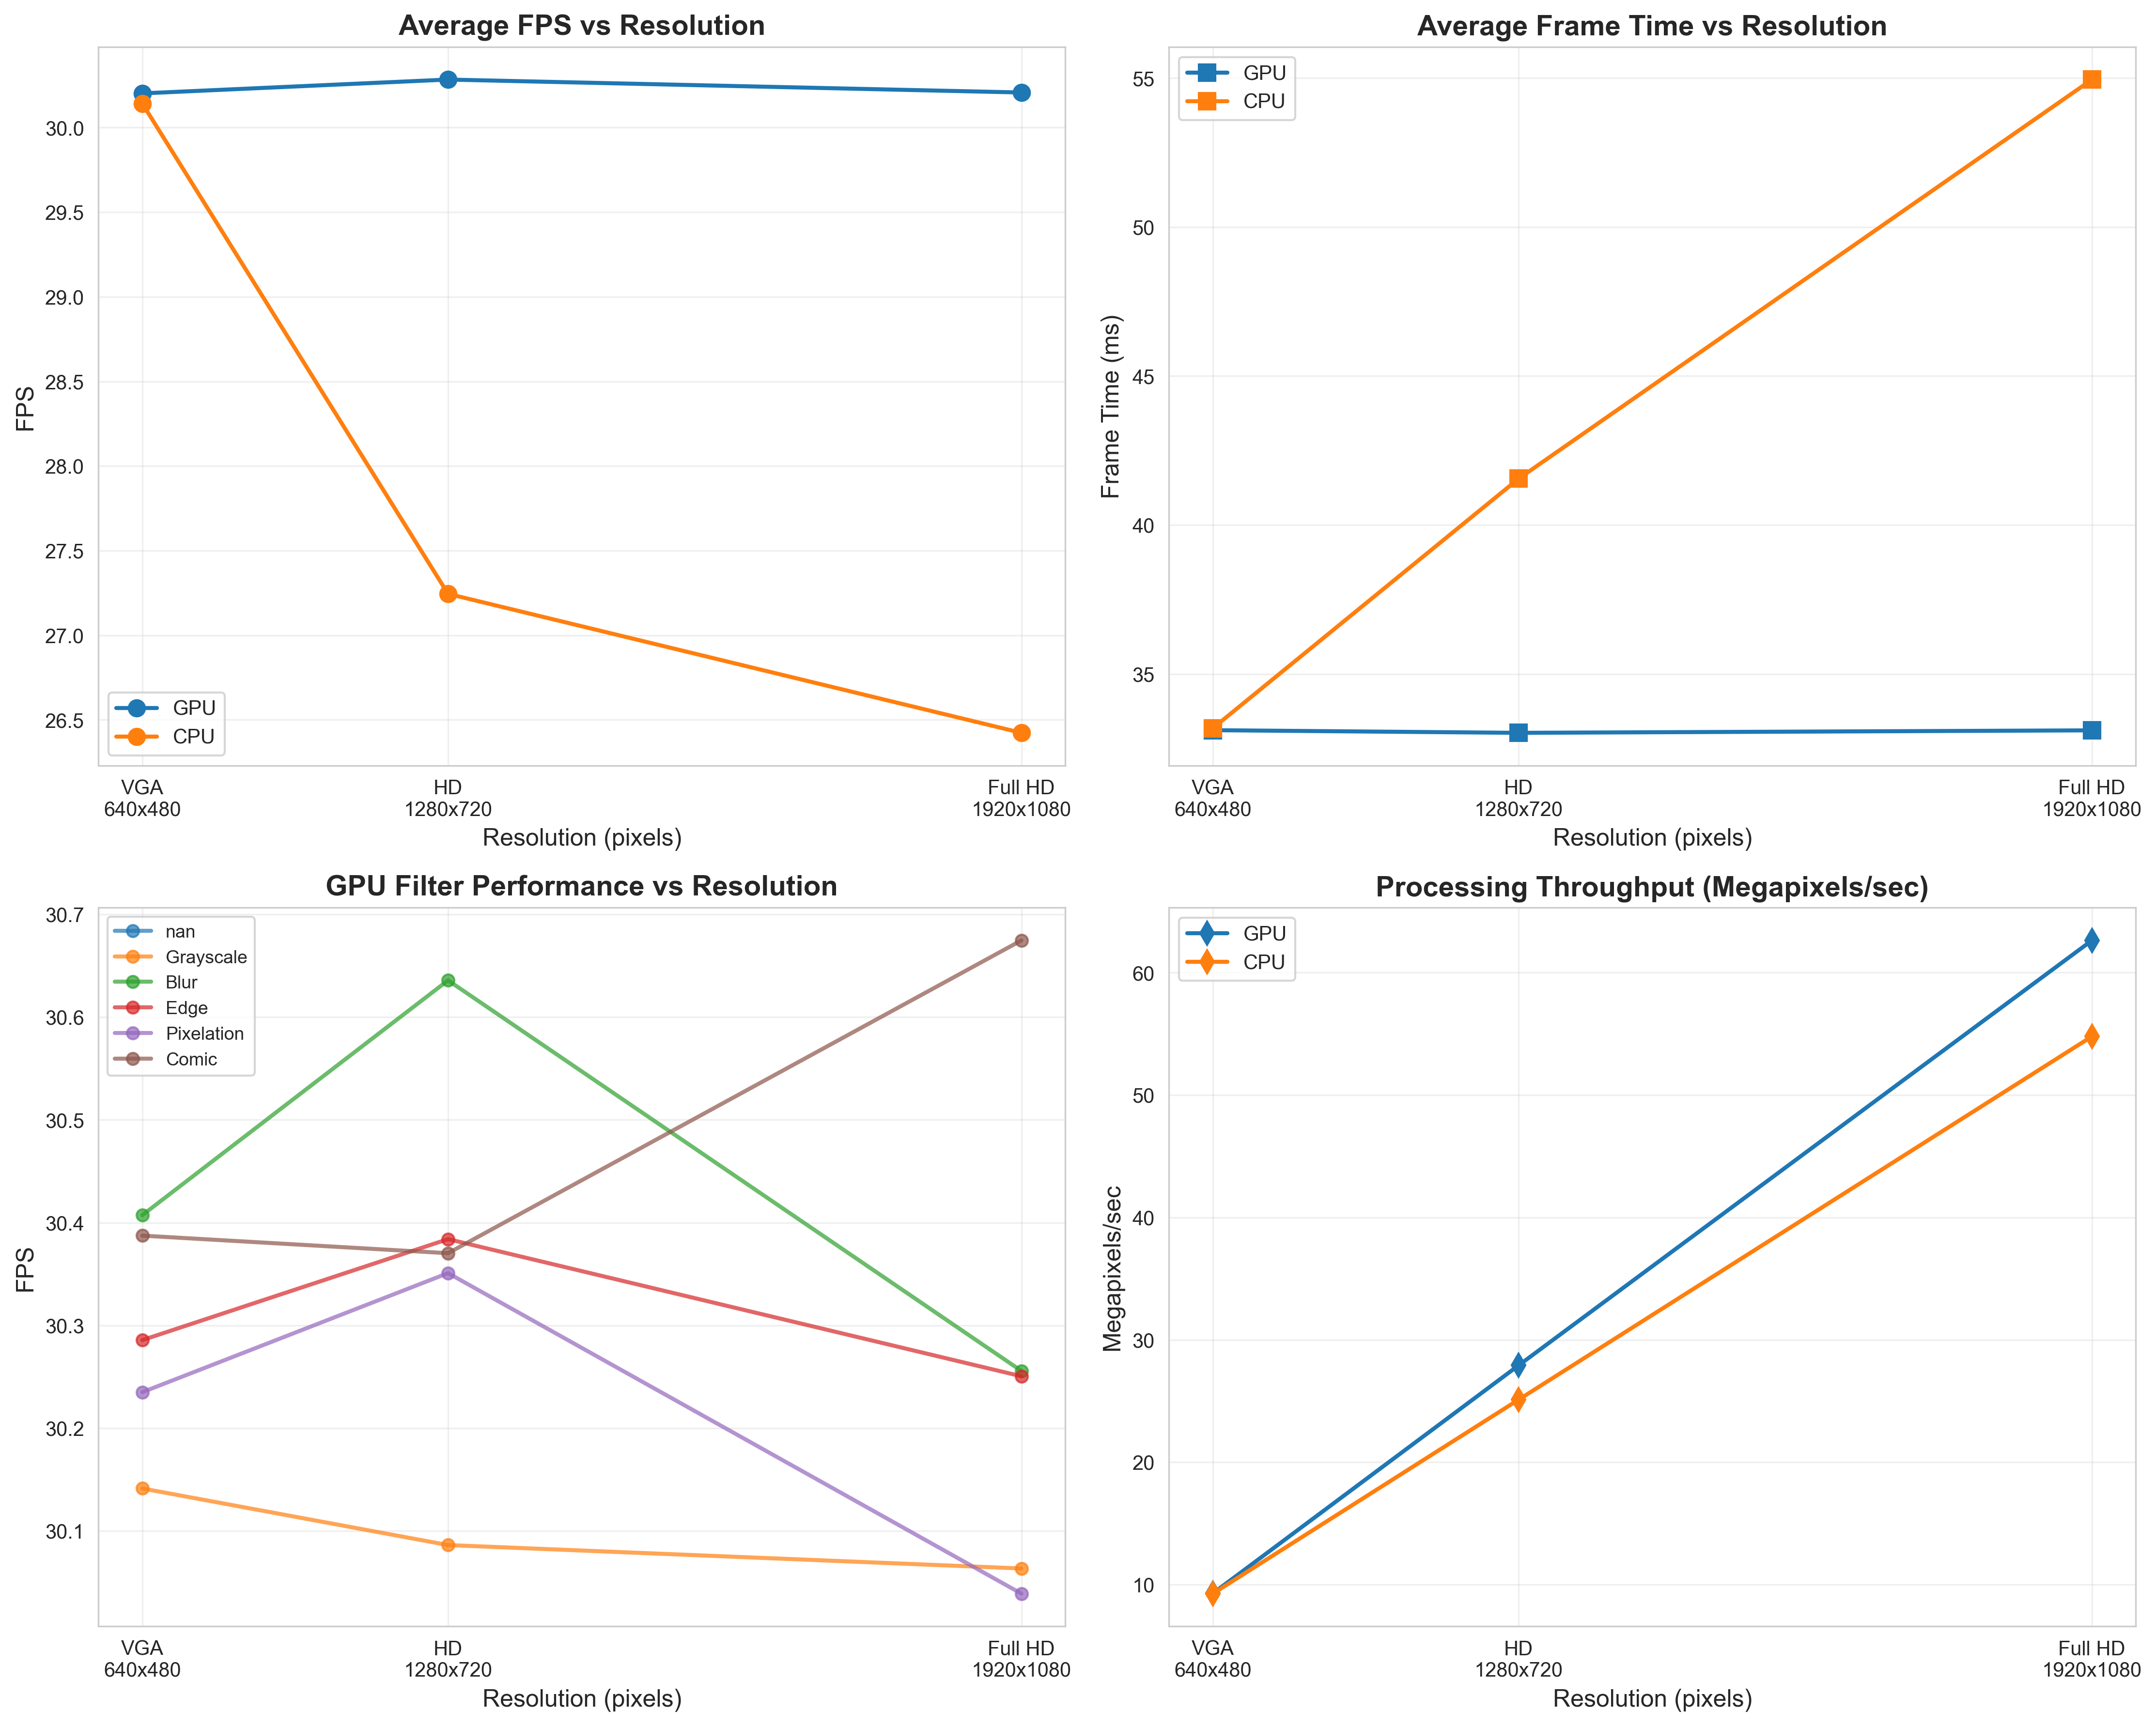
\includegraphics[width=0.9\textwidth]{../data/plots/resolution_impact.png}
    \caption{Performance across different resolutions}
    \label{fig:resolution_impact}
\end{figure}

% TODO: Add analysis text here

\subsection{Performance Tables}

\subsubsection{GPU Speedup Factors resolution}
\begin{table}[H]
    \centering
    \caption{GPU speedup over CPU for each filter}
    \label{tab:speedup}
    \begin{tabular}{lc}
        \toprule
        Filter & Speedup Factor \\
        \midrule
        None & 0 \\
        Grayscale & 0.9911051151304507 \\
        Blur & 0.9832661231455018 \\
        Edge Detection & 0.9905437890552572 \\
        Pixelation & 0.9921230970698969 \\
        Comic Art & 5.056022571870571 \\
        \bottomrule
    \end{tabular}
\end{table}

\subsubsection{GPU Speedup Factors transforms}
\begin{table}[H]
    \centering
    \caption{GPU speedup over CPU for each filter}
    \label{tab:speedup}
    \begin{tabular}{lc}
        \toprule
        Filter & Speedup Factor \\
        \midrule
        None & 0 \\
        Grayscale & 0.9925609416695316 \\
        Blur & 0.9892095840826678 \\
        Edge Detection & 0.9861874029899519 \\
        Pixelation & 0.9961871093584084 \\
        Comic Art & 4.996309606519084 \\
        \bottomrule
    \end{tabular}
\end{table}

\section{Analysis and Discussion}

\subsection{CPU vs GPU Performance}
\subsubsection{Unexpected GPU Performance}
The most striking finding from the benchmarks is that GPU processing shows no performance advantage over CPU processing for most filters, and in some cases performs slightly worse (speedup factors of 0.98-0.99). This is somewhat counterintuitive, and some of the factors that could lead to this are being listed below:
\begin{itemize}
    \item \textbf{Memory Transfer Overhead}: Each of the frames are going from system RAM to GPU memory as a texture. Now for the tested resolutions all the way up to 1920×1080, this transfer time dominates the processing time, negating any computational advantages.
    \item \textbf{Simple Filter Complexity}: Most implemented filters (grayscale, blur, edge detection) are relatively simple operations. The computational load is low enough that the CPU can handle them efficiently without the need for parallel GPU processing. Hardware used is a M4 Pro chip with 16 core CPU.
    \item \textbf{Webcam Framerate Limitation}: The camera operates at approximately 30 FPS maximum, creating a bottleneck that prevents either of the processing methods from showing its full potential.
\end{itemize}

\subsection{Filter Complexity}
\subsubsection{Filter Performance Characteristics}
All filters except Comic Art maintain similar performance (~30 FPS on both CPU and GPU), suggesting:
\begin{enumerate}
    \item The camera capture rate is the primary bottleneck
    \item Simple filters don't stress either processing architecture
    \item More complex filters (Comic Art) reveal processing architecture differences, which is therefore also the most interesting filter
\end{enumerate}

\subsection{Resolution Impact}
From the resolution benchmark data (VGA to Full HD, representing a 6.75 times pixel increase):
\begin{itemize}
    \item \textbf{FPS Variation}: Performance drops for the CPU are very evident, compared to the GPU, when upscaling resolution, performance worsens. Like seen in \ref{fig:resolution_impact}. This is because the CPU has to handle more data without the parallel processing capabilities of the GPU.
\end{itemize}

\subsubsection{Implications}
The results suggest that for higher resolutions, GPU processing becomes more advantageous due to its ability to handle larger data sets more efficiently through parallelism. This is especially true for more complex filters, where the computational load is higher. 

\subsection{Transform Overhead}
\subsubsection{GPU Transform Efficiency}
Geometric transformations on the GPU (vertex shader operations) show negligible overhead:
\begin{itemize}
    \item Transformations are mathematical operations on 4 vertices per frame
    \item GPU vertex processors handle these operations trivially
    \item No measurable FPS difference between transformed and non-transformed rendering
\end{itemize}

\subsubsection{CPU Transform Cost}
CPU transformations using \texttt{warpAffine()} introduce overhead:
\begin{itemize}
    \item Requires interpolation calculations for every pixel
    \item Memory access patterns become less cache-friendly
    \item Additional processing step in the pipeline
\end{itemize}

However, the overhead remains minimal (~1-2\% FPS reduction) due to:
\begin{itemize}
    \item Camera framerate limiting overall throughput
    \item Efficient OpenCV implementation
    \item Simple affine transformations (not perspective warps)
\end{itemize}

\subsection{Shader design and its limitations}

\subsection{Showcasing filters}


\end{document}